\chapter{Evaluación del sistema}

Para la evaluación del transmisor, nos pusimos como objetivo final lograr la transmision exitosa hacia un televisor comercial homologado por el LATU. En ese camino, nos propusimos una serie de objetivos de más corto alcance. Desarrollamos en este capítulo los resultados de las pruebas realizadas con \textit{gr-isdbt-tx}.

Primero, nos habíamos propuesto lograr la decodificación con \textit{gr-isdbt} dentro del mismo flowgraph (eso es, una prueba del sistema punta a punta trasmitiendo en condiciones ideales). Luego, nos propusimos una situación en la que una PC ejecuta el transmisor, enviando la señal a través del USRP, y otra computadora hace lo propio con el receptor \textit{gr-isdbt}. Esto le agrega a la prueba anterior, el desafío de la puesta en el aire y decodificación de la señal ruidosa.

Por último, nos planteamos el objetivo final, la decodificación contra un televisor comercial. En este capitulo desarrollamos estas pruebas, y el nivel de éxito que alcanzó cada una.

En virtud de poder asegurar si se cumplen o no esos objetivos es necesario contar con herramientas que permitan medir de alguna manera la calidad de una señal digital. Existen varios indicadores de calidad en una transmisión digital, en este caso nos basaremos en dos de ellos que son ampliamente utilizados y proporcionan una medida cuantitativa de la calidad de la señal. A continuación definiremos y el \textit{Bit Error Rate} (BER), y el \textit{Modulation Error Rate} (MER).

\section{Indicadores de calidad de una señal}
\subsection{Bit Error Rate (BER)}
El estándar ISDB-T en su etapa de codificación de canal hace uso de una combinación de códigos de Reed-Solomon junto con códigos convolucionales, ambos están orientados a la corrección de errores de bits. En recepción se utilizan los decodificadores Viterbi y Reed-Solomon. Resulta importante cuantificar esos errores que se producen así como conocer la proporción de ellos que se han podido recuperar. Es de interés conocer tanto la cantidad de errores que hay antes del Viterbi, luego del Viterbi (antes del Reed-Solomon) y luego del Reed-Solomon.

Se define la tasa de error de bits (BER) como el cociente entre la cantidad de bits erróneos que se recibieron y la cantidad de bits totales.

Para realizar una medición del BER hay que elegir un intervalo de tiempo determinado sobre el cual se va a promediar. En pruebas de aceptación de equipos comerciales se suelen realizar tests que duran varias horas, mientras que para pruebas de monitoreo los tests suelen ser de algunos minutos.



\subsection{Modulation Error Rate (MER)}
La tasa de error de modulación (MER) es una medida de la suma de todas las interferencias que afectan a una señal de TV digital. Para el cálculo del MER se registran todos los símbolos recibidos y sus desviaciones $(\delta I_{j}, \delta I_{j})$ respecto a su posición teórica, donde el subíndice $j$ corresponde al símbolo j-ésimo. Finalmente el MER corresponde al cociente entre la suma de los módulos de los símbolos teóricos sobre el módulo de la suma de los vectores de error formado por los $(\delta I_{j}, \delta I_{j})$. Es común encontrarlo expresado en escala logarítmica. 


\begin{equation}
MER = 10 \log_{10} \left( \dfrac{\sum_{j = 0}^{N-1} I_{j}^{2}+ Q_{j}^{2}}{\sum_{j = 0}^{N-1}\delta I_{j}^{2}+\delta Q_{j}^{2}} \right )
\end{equation}


Tener un MER alto indica una buena calidad en la señal, para los equipos comerciales se considera un MER de 35dB como muy bueno. Las señales recibidas en un hogar a través de una antena instalada en el techo tienen un MER que se ubica entre los 20dB y 30dB aproximadamente. 

El MER se puede medir de varias maneras según lo que interese considerar. Es común muy calcular el MER para cada una de las capas por separado, pero también es posible considerar todas las señales incluyendo las portadoras piloto. Tener en cuenta las portadoras piloto para el cálculo del MER puede provocar que el promedio esté un poco por encima del MER de las tres capas por separado.


\section{Pruebas sobre gr-isdbt}

Considerando que realizamos la mayoría del desarrollo contrastando los bloques del transmisor contra los de gr-isdbt, no parecería en principio un desafió mayor lograr la decodificacion punta a punta. Pero en si, lo es, y eso es parte de la potencia del desarrollo con código abierto desde el otro lado. 

Como receptor, \textit{gr-isdbt} ha sido sometido a una diversidad de pruebas con resultados satisfactorios, por lo tanto, podemos considerarlo como una simulación de un televisor comercial válida. Es en ese punto en el que comenzamos las pruebas. Dentro de un entorno controlado, el transmisor \textit{gr-isdbt-tx} conectado a la entrada del receptor \textit{gr-isdbt}.





\subsubsection{Pruebas sobre el flowgraph}

En este caso ideal, donde todo funciona dentro de un mismo flowgraph y no hay variabilidad de las muestras transmitidas, el transmisor se comporta de forma perfecta. Sí encontramos, consumo excesivo de CPU en algunos bloques, en parte debido a problemas de optimización del código.

Para la prueba se utilizó un BTS constituido por tres capas jerárquicas donde se destina un segmento para la capa A y seis segmentos para las capas B y C respectivamente, todas en moduladas en 64QAM. Tanto la tasa de código convolucional como la profundidad del entrelazamiento temporal son las mismas para las tres capas y es de 1/2 y 8 respectivamente. 

\begin{figure}[!h]
	\centering
	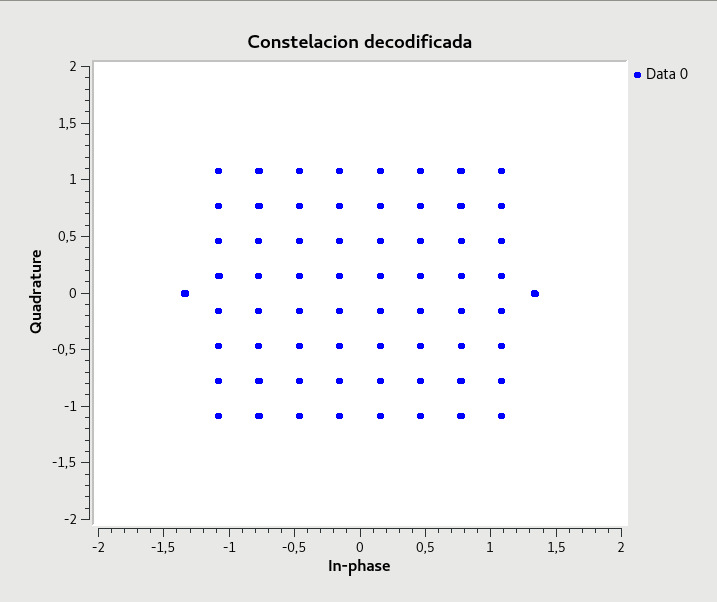
\includegraphics[scale=0.5]{figuras/cap06/const_rec}
	\caption{\label{f:const_rec} Constelación en recepción. Caso ideal.}
\end{figure}

Como se puede ver en la figura \ref{f:const_rec}, el receptor \textit{gr-isdbt} se sincroniza perfectamente con la señal transmitida, y en la constelación de recepción, vemos la misma constelación que en transmisión. Esto no debe sorprender, ya que en esta prueba, el canal esta representado por un cable ideal. En la misma figura se puede apreciar las modulaciones 64QAM utilizada para las portadoras de datos y BPSK para las señales piloto. 

Recibir la constelación perfecta en \textit{gr-isdbt} significa varias cosas. Por un lado el cuadro OFDM está siendo conformado correctamente del lado del transmisor, y por otro lado se está decodificando correctamente las portadoras piloto (SP, TMCC y piloto continuo). Además el receptor entiende perfectamente la información contenida en la TMCC, es decir que su contenido es el correcto y pasa satisfactoriamente los chequeos de paridad.

Podemos asegurar que esta prueba constituye un éxito dado que en el otro extremo de \textit{gr-isdbt} se logró obtener cada una de las tres capas jerárquicas transmitidas sin algún tipo de error.

A esta prueba se le agregó un bloque \verb|Channel Model| que simula un canal que agrega ruido blanco gaussiano y cuyos parámetros potencia de ruido, offset de frecuencia y respuesta al impulso son configurables. Se observó que el decodificador Reed-Solomon a partir de un cierto nivel de ruido deja de funcionar, sin embargo la TMCC continúa decodificándose correctamente incluso para niveles de ruido más altos. La tabla \ref{t:resultados_errores} resume los resultados obtenidos para distintos valores de la potencia de ruido $N$.

\begin{table}[h!]
	\centering
	\begin{tabular}{|c|c|c|}
		\hline
			& \textbf{N = 9} & \textbf{N = 10}\\
		\hline
		\textbf{BER Reed-Solomon} & 0.0065 & 0.49\\
		\hline
		\textbf{BER Viterbi}		& 0.051 & 0.064\\
		\hline
	\end{tabular}
	\caption{\label{t:resultados_errores} Valores de BER en los bloques correctores de errores.}
\end{table} 

Para valores $N < 9$ el BER es prácticamente el mismo, para cualquier $N$. Se observa que a partir de $N = 10$ el BER en el bloque Reed Solomon se dispara enormemente, alcanzando una tasa de la mitad de los bits erróneos. Esto pone de manifiesto la gran capacidad que tienen los códigos de Reed-Solomon pero si se supera el umbral de capacidad, su desempeño cae drásticamente. Para dar una idea de cómo resulta esto en términos de calidad de la imagen recibida, la figura \ref{f:calidad_imagen} muestra los resultados para los casos en que $N = 9$ y $N = 10$.

\begin{figure}[!h]
	\centering
	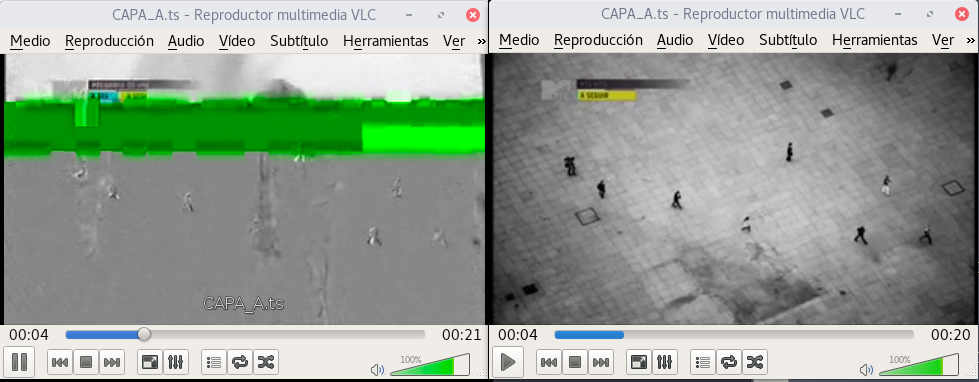
\includegraphics[scale=0.4]{figuras/cap06/calidad_imagen}
	\caption{\label{f:calidad_imagen} Calidad de la imagen recibida para $N=10$ (izquierda) y $N=9$ (derecha).}
\end{figure}

\subsubsection{Pruebas en el aire}

Realizamos la misma prueba de antes con \textit{gr-isdbt} como receptor, pero en lugar de simular un canal en GNU Radio, utilizamos el aire y transmitimos en una linea vista de un metro de distancia.

El resultado fué interesante. Si bien no es posible decodificar las señales todavía, intermitentemente es posible observar la constelación en recepción. 

Entendemos que tenemos algún problema de sincronismo, surgido seguramente por el uso del USRP. Dado que es el único cambio entre la prueba anterior y esta.
 

\section{Pruebas sobre televisores comerciales}

Si bien las pruebas contra \textit{gr-isdbt} con canal inalámbrico no fueron del todo satisfactorias, se intentó transmitir hacia un televisor comercial compatible con ISDB-T. 

Esta prueba resultó exitosa, lográndose ver con excelente calidad las tres capas jerárquicas transmitidas. Se probó transmitir sin línea de vista, moviendo la antena transmisora, y a una distancia de 5 metros. En todos los casos el televisor reproduce la imágen sin problema.

Sí se puede notar alguna imperfección en cuanto a la fluidez del video en el televisor pero sin algún tipo de pixeleo o congelamiento de la imágen. Las pruebas se realizaron durante varias horas a lo largo de cuatro días, y en ningún momento se perdió comunicación con el televisor.



\section{Pruebas con equipos analizadores de TV}

De las pruebas anteriores surgen varias hipótesis sobre la recepción intermitente con \textit{gr-isdbt} y las imperfecciones en la recepción con TV comercial. Podría deberse tanto a un desajuste en la tasa de muestreo del lado del transmisor, así como también un incorrecto manejo de los equipos USRP o limitaciones por sus especificaciones de diseño.

Se tuvo la posibilidad de acceder a un equipo ETH de Rohde \& Schwarz, propiedad de la Unidad Reguladora de Comunicaciones, que es capaz de analizar señales de TV compatible con ISDB-T. 

\begin{figure}[!h]
	\centering
	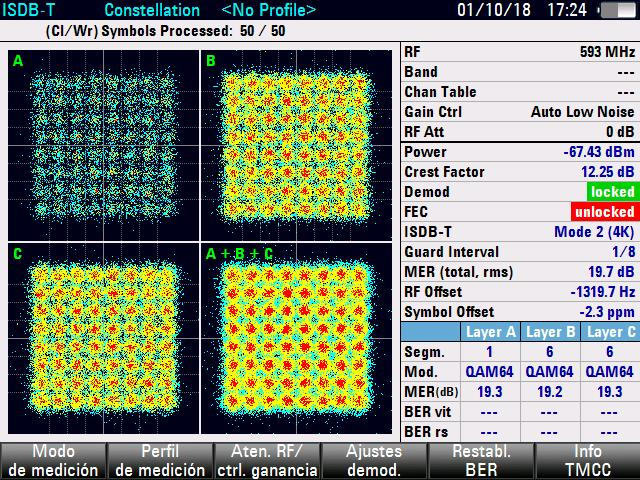
\includegraphics[scale=0.6]{figuras/cap06/constelacion_eth}
	\caption{\label{f:calidad_imagen} Constelación de las tres capas jerárquicas tomadas con el analizador ETH de Rohde \& Schwarz.}
\end{figure}

Con este instrumento se pudo observar claramente las constelaciones de las tres capas jerárquicas pero con demasiado ruido. También se observó que la señal presenta una variabilidad bastante grande del offset en frecuencia. Esto quizás sea parte de la causa de la mala recepción en \textit{gr-isdbt}.

